\documentclass[smallextended,natbib,runningheads]{svjour3}
%
\journalname{Annals of the Institute of Statistical Mathematics}
%
\smartqed  % flush right qed marks, e.g. at end of proof
%
\usepackage{graphicx}
%
% \usepackage{times}
% \usepackage[LY1]{fontenc}
% \usepackage[LY1,mtbold]{mathtime}
% %
% \usepackage{marvosym}
% \newcommand{\envelope}{(\raisebox{-.5pt}{\scalebox{1.45}{\Letter}}\kern-1.7pt)}
% %
% %\usepackage{mathptmx}
% \usepackage{times}
% \usepackage[LY1]{fontenc}
% \usepackage[LY1,mtbold]{mathtime}
% \usepackage{biograph}
% %
% \input{glov3.doi}
% \let\SprJLogo=\relax
% \DOIyear{2002}
% \OFyear{2003}
% \DOImsnr{6789}
% \journalnumber{10463}
% \idline{12: 345--678}{345}
% \papertype{generic article}
%
% \usepackage{mathptmx}      % use Times fonts if available on your TeX system
%
% insert here the call for the packages your document requires
%\usepackage{latexsym}
% etc.
%
% please place your own definitions here and don't use \def but
% \newcommand{}{}
%

\usepackage{amsmath,amssymb}
\usepackage{booktabs}
\usepackage{xcolor}
\usepackage{url}
\graphicspath{{../presentation/Images/final/}}

\newcommand{\todo}[1]{\textcolor{red}{\textbf{TODO:} #1}}
\newcommand{\draftnote}[1]{\textcolor{blue!70!black}{\textbf{Draft note:} #1}}
\newcommand{\R}{\mathbb{R}}
\newcommand{\given}{\,\middle|\,}
\newcommand{\Haus}{\mathcal{H}}
\begin{document}

\title{Bayesian Inference under Maximum Likelihood Constraints
%\thanks{Grants or other notes
%about the article that should go on the front page should be
%placed here. General acknowledgments should be placed at the end of the article.}
}
\subtitle{What Does the Maximum Likelihood Estimator Reveal?}

%\titlerunning{Short form of title}        % if too long for running head

\author{Antoine Luciano \and Shlok Mishra \and Christian P. Robert
}

%\authorrunning{Short form of author list} % if too long for running head

\institute{Christian P. Robert \at
              CEREMADE, Université Paris Dauphine - PSL \\
              \email{xian@ceremade.dauphine.fr}           %  \\
%             \emph{Present address:} of F. Author  %  if needed
           \and
           S. Author \at
              second address
}

\date{Received: date / Revised: date}
% The correct dates will be entered by the editor


\maketitle

\draftnote{Review status, 12 October 2026: this is an earlier manuscript draft.
Its narrative and figures have not been updated to the latest selected-MLE
corrections and full latent-chain diagnostics. The current collaborator account
is \texttt{docs/research/location\_only\_meeting\_brief.md}, with links to the
frozen evidence. Read that note before interpreting the results below as the
current validation status.}

\begin{abstract}
Releasing an estimator rather than a dataset is a common form of statistical
compression, but it does not by itself answer either an inferential or a
privacy question: how much information about the parameter and about the
unreleased observations remains in the estimator?  We study Bayesian inference
when the released object is a maximum likelihood estimator (MLE).  Outside
exponential families, the MLE is generally not sufficient, and exact
conditioning restricts the latent data to a level set of the estimator map.  We
formulate the resulting posterior using the coarea formula and develop
data-augmentation Markov chains that alternate between an ordinary parameter
update and model-specific moves of the latent data along this level set.  Our
main construction is a pairwise Gibbs--Metropolis sampler for location models.
For the Student distribution it uses the transformed score
$z=y/(k+y^2)$, preserves the released score value exactly, and explicitly
samples both inverse branches of the transformation.  The same formulation
also exposes an important distinction between conditioning on a score root and
conditioning on the selected MLE.  We use smooth and non-smooth location
models to study posterior information loss, disclosure about latent extremes,
and the practical cost of exact constraint preservation.

\draftnote{This is a working abstract.  Replace the last two sentences with
the final theorem and simulation findings once the exact-MLE correction and
the production experiments are frozen.}

\keywords{maximum likelihood \and insufficient summaries \and robust
estimation \and data privacy \and constrained Markov chain Monte Carlo \and
manifold sampling}
\end{abstract}

\section{Introduction}
\label{sec:introduction}

The maximum likelihood estimator (MLE) is one of the most widely reported
summaries in parametric statistics.  Under familiar regularity conditions it
is consistent and asymptotically efficient, and its dimension is usually the
dimension of the parameter rather than the sample size.  An MLE can therefore
look like a natural object to release when the full dataset is confidential or
too cumbersome to share.  Compression, however, is not a privacy guarantee.
Even a low-dimensional statistic can alter beliefs about an individual or a
hidden feature of the sample.  Conversely, the statistic can discard
information that matters for subsequent inference.

This paper begins with two related questions.  If only the value
$\hat\theta=t^\star$ is observed, what is the posterior distribution of
$\theta$?  And what does the same release reveal about unreleased aspects of
the sample, such as the presence of extreme observations?  The first question
measures the inferential value retained by the MLE.  The second measures
\emph{inferential disclosure}: the prior-to-posterior change in beliefs about a
latent data feature.  This use of privacy language is deliberately narrower
than differential privacy, which is a worst-case stability property of a
randomized release mechanism \citep{dwork2006}.  An unrandomized MLE is not
claimed to satisfy differential privacy.

The answer depends critically on the statistical model.  When the MLE is in
one-to-one correspondence with a sufficient statistic, conditioning on the MLE
is equivalent to conditioning on that statistic, and no Bayesian information
about the parameter is lost.  The normal location model with known variance is
our canonical zero-loss example.  Outside such cases, the MLE is a
coarsening of the full experiment.  In Blackwell's ordering it cannot be more
informative than the complete data \citep{blackwell1953}, but this exact order
does not say whether the loss is practically important for a specified family
of decisions, priors, and sample sizes.

Robust estimation makes the question especially interesting.  An
$M$-estimator solves an equation of the form
\begin{equation}
  \sum_{i=1}^n \psi(x_i-t)=0.
  \label{eq:m_equation_intro}
\end{equation}
Bounded scores limit the contribution of a single large residual, and
redescending scores make that contribution vanish in the far tail.  This is a
central mechanism in robust estimation \citep{huber1964}.  In the informal
phrase motivating this work, ``the tails are less important'' for the point
estimate.  But this phrase needs qualification.  It concerns the sensitivity
of the estimator, not the probability of extreme latent samples conditional on
the estimator.  Many central and tail-heavy datasets can satisfy the same
estimating equation.  The conditional distribution over these compatible
datasets is precisely what makes both the information-loss and disclosure
questions non-trivial.

We use the phrase \emph{weak sufficiency} for the working hypothesis that, in
some regimes, little of practical relevance is lost by replacing $X$ with
$\hat\theta(X)$ even though classical sufficiency fails.  This is not a new
factorization criterion.  We operationalize it through posterior distances and
decision-specific regret, averaged over repeated datasets.  The hypothesis may
hold in central, moderate-sample regimes and fail for tail-sensitive
functionals or small samples.  Stating the question this way prevents a close
posterior mean from being mistaken for general sufficiency.

Computationally, exact conditioning on a continuous statistic is a geometric
problem.  For a regular value $t^\star$, the compatible samples form the level
set
\begin{equation}
  \mathcal M_{t^\star}=\{x:\hat\theta(x)=t^\star\},
  \label{eq:mle_level_set_intro}
\end{equation}
which is typically a lower-dimensional manifold and therefore has Lebesgue
measure zero in the ambient data space.  Approximate Bayesian computation
(ABC) replaces equality by a tolerance event, introducing a bandwidth and an
approximation error \citep{marin2012}.  Our aim is instead to work on the level
set itself.

Sampling on implicitly defined manifolds is now supported by a growing body of
work: constrained Hamiltonian methods, projection-based Metropolis kernels,
and constrained inference for differentiable simulators
\citep{brubaker2012,graham2017,zappa2018,lelievre2019}.  These methods clarify
the measure correction, projection, and reversibility issues that arise on a
level set.  They are general, but generality has a cost.  A model-specific
transition can exploit the algebra of an estimating equation, avoid repeated
nonlinear projections, and remain applicable when the constraint is
non-smooth.  This motivates our augmented Gibbs strategy, following the broad
data-augmentation principle of \citet{tanner1987}.

We augment the parameter by a latent dataset and alternate between

\begin{enumerate}
    \item a conventional update of $\theta$ conditional on the current latent
    dataset $x$; and
    \item model-specific updates of $x$ conditional on $\theta$ that preserve
    the released estimating equation.
\end{enumerate}

Our main example is Student location with known scale and degrees of freedom.
Its score is bounded and redescending.  Pairwise latent updates become simple
after transforming each residual by its score contribution, but the
transformation has two inverse branches.  Correct sampling must explore both
the central and tail branches.  This mechanism also makes the privacy question
visible: a very large residual can have nearly the same score contribution as
a residual close to zero.

There is one distinction that the paper must keep explicit.  Satisfying the
score equation at $t^\star$ is necessary for $t^\star$ to be an interior MLE,
but it is not always sufficient: the root may be a minimum or a non-selected
local maximum.  Moreover, the coarea density induced by the estimator map
contains a Jacobian that is not, in general, the same as the Jacobian induced
by the score map.  Section~\ref{sec:target} derives the correction.  The current
production Gibbs and RATTLE implementations target the score-conditioned
level set; converting them into exact selected-MLE samplers is therefore a
central item in the paper's theory and experimental roadmap.

The intended contributions are:
\begin{enumerate}
  \item a precise formulation of posterior inference and inferential disclosure
  from a released estimator;
  \item a coarea-based separation of estimator conditioning from
  score-equation conditioning;
  \item a branch-aware pairwise Gibbs--Metropolis construction for robust
  location models; and
  \item a simulation study comparing inference from the MLE with full-data
  Bayes and comparing specialized Gibbs transitions with generic constrained
  samplers under a fixed computational budget.
\end{enumerate}

\draftnote{The remainder is intentionally a hybrid of prose and a research
roadmap.  Blue notes identify claims that should not enter the final paper
until the corresponding derivation or experiment is complete.}

\section{Conditioning on a released estimator}
\label{sec:target}

\subsection{The coarea target}

Let $X\in\R^n$ have density $f_\theta(x)$ under parameter
$\theta\in\Theta\subseteq\R^p$, with prior density $\pi_0(\theta)$, and let
$T:\R^n\to\R^p$ denote the released estimator.  Suppose that $t$ is a regular
value of $T$.  Write
\[
  J_T(x)=\left\{\det[D T(x)D T(x)^\mathsf T]\right\}^{1/2}.
\]
The coarea formula gives the sampling density of the released statistic as
\begin{equation}
 p_T(t\mid\theta)
 =\int_{\mathcal M_t}\frac{f_\theta(x)}{J_T(x)}
 \,d\Haus^{n-p}(x),
 \qquad \mathcal M_t=T^{-1}(t).
 \label{eq:coarea_likelihood}
\end{equation}
Consequently, a convenient augmented target, with respect to
$d\theta\,d\Haus^{n-p}(x)$, is
\begin{equation}
 \Pi(d\theta,dx\mid T=t^\star)
 \propto
 \pi_0(\theta)\frac{f_\theta(x)}{J_T(x)}
 \mathbf 1\{x\in\mathcal M_{t^\star}\}
 \,d\theta\,d\Haus^{n-p}(x).
 \label{eq:augmented_exact_target}
\end{equation}
This answers the earlier augmentation question: joint sampling is feasible in
principle, but only after specifying the correct surface measure and a Markov
kernel that can move within its support.

\subsection{Estimator maps versus estimating equations}
\label{sec:score-versus-mle}

Suppose $T(x)$ is locally defined by a smooth estimating equation
\[
 C(x,T(x))=0,\qquad C:\R^n\times\R^p\to\R^p,
\]
and $D_tC$ is non-singular.  Implicit differentiation yields
\[
 DT(x)=-[D_tC(x,T(x))]^{-1}D_xC(x,T(x)).
\]
On a branch on which the estimating equation selects the released estimator,
equation~\eqref{eq:augmented_exact_target} is therefore proportional to
\begin{equation}
 \pi_0(\theta)f_\theta(x)
 \frac{|\det D_tC(x,t^\star)|}
 {\left\{\det[D_xC(x,t^\star)D_xC(x,t^\star)^\mathsf T]\right\}^{1/2}}
 \mathbf 1\{T(x)=t^\star\}.
 \label{eq:estimating_equation_correction}
\end{equation}
For a likelihood score, $D_tC$ is the observed Hessian.  Conditioning only on
$C(x,t^\star)=0$ instead gives the denominator in
\eqref{eq:estimating_equation_correction}, but not the Hessian numerator or the
indicator selecting the relevant root.  The distinction disappears in some
monotone-score models, or the extra factor may simplify, but it cannot be
discarded by default.

\draftnote{Priority theory task: verify equation
\eqref{eq:estimating_equation_correction} for each model and estimator
convention, including the global-MLE selection event.  For Student location,
quantify separately the Hessian correction and the multiple-root correction.
The repository already contains a score-root versus selected-MLE diagnostic;
it does not yet settle the Hessian factor.}

\subsection{Information retained and information disclosed}

Let $\Pi_X=\pi(\theta\mid X)$ and
$\Pi_T=\pi(\theta\mid T(X))$.  We will quantify loss with several complementary
summaries:
\begin{equation}
 \mathcal L_d=\mathbb E\{d(\Pi_X,\Pi_T)\},
 \label{eq:posterior_loss}
\end{equation}
where $d$ may be a Wasserstein distance, a difference in posterior quantiles,
or a ratio of interval widths, and with decision-specific Bayes-risk regret
when a loss function is scientifically meaningful.  Equality of posterior
means alone is not enough to establish weak sufficiency, especially in
heavy-tailed settings.

For disclosure, let $h(X)$ be a latent feature, for example
$h_c(X)=\mathbf 1\{\max_i|X_i-t^\star|>c\}$.  At release value $t$ define
\begin{equation}
 \Delta_h(t)=
 \Pr\{h(X)=1\mid T(X)=t\}-\Pr\{h(X)=1\}.
 \label{eq:privacy_shift}
\end{equation}
This is a model- and prior-dependent belief shift, not a universal privacy
parameter.  We will report both signed shifts and probability ratios over a
range of thresholds, together with the prior predictive baseline.

\section{Location models and robust score geometry}
\label{sec:models}

Consider a location family
\[
  X_i=\mu+\varepsilon_i,\qquad \varepsilon_i\overset{\mathrm{iid}}\sim g,
  \qquad \mu\sim\pi_0.
\]
For a differentiable log density, write $\psi(y)$ for the location score up to
an irrelevant positive constant.  A released root $\mu^\star$ imposes
\begin{equation}
 C(x;\mu^\star)=\sum_{i=1}^n\psi(x_i-\mu^\star)=0.
 \label{eq:location_constraint}
\end{equation}
The examples in the computational study are summarized below.

\begin{table}[t]
\centering
\caption{Working location models.  ``Tail behavior'' describes the score, not
the sampling distribution.}
\label{tab:models}
\small
\begin{tabular}{p{0.17\textwidth}p{0.19\textwidth}p{0.20\textwidth}p{0.29\textwidth}}
\toprule
Model & Released estimator & $\psi(y)$ & Constraint geometry \\
\midrule
Normal, known variance & sample mean & $y$ & linear, sufficient \\
Logistic, known scale & score root & $\tanh(y/2)$ & smooth, monotone \\
Student $t_k$, known scale & selected score root & $y/(k+y^2)$
  & smooth, two branches \\
Laplace, known scale & sample median & $\operatorname{sign}(y)$
  & non-smooth, order based \\
\bottomrule
\end{tabular}
\end{table}

The Student case is the main methodological example.  With known degrees of
freedom $k$ and unit scale,
\begin{equation}
 f_\mu(x)=c_k\left(1+\frac{(x-\mu)^2}{k}\right)^{-(k+1)/2},
 \qquad \mu\sim N(m_0,s_0^2).
 \label{eq:student_model}
\end{equation}
For $y=x-\mu^\star$,
\[
 \psi(y)=\frac{y}{k+y^2},\qquad
 \psi'(y)=\frac{k-y^2}{(k+y^2)^2}.
\]
The score is largest in magnitude at $|y|=\sqrt{k}$ and tends to zero as
$|y|\to\infty$.  Thus the same small value of $z=\psi(y)$ can arise from a
central residual or an extreme residual.  The two inverse branches are
\begin{equation}
 y_\pm(z)=\frac{1\pm\sqrt{1-4kz^2}}{2z},
 \qquad |z|<\frac{1}{2\sqrt{k}},
 \label{eq:student_inverse}
\end{equation}
with the $z=0$ limit handled separately.  This algebra drives the specialized
sampler and the heavy-tail diagnostics.

\section{A constrained augmented Gibbs sampler}
\label{sec:gibbs}

\subsection{Two-block construction}

For the augmented target, one iteration consists of:
\begin{enumerate}
  \item update $\mu$ from a Markov kernel invariant for
  $\pi(\mu\mid x)\propto\pi_0(\mu)\prod_i f_\mu(x_i)$; and
  \item update the latent data from a kernel invariant for their conditional
  distribution on the constraint set.
\end{enumerate}
The implementation uses a random-walk Metropolis update for the scalar
parameter.  The surface/Jacobian factor depends on $x$ and the released value,
so it drops out of the first block.  The second block is model dependent.

\subsection{Student pair update}
\label{sec:student_pair_update}

Set $y_i=x_i-\mu^\star$ and $z_i=\psi(y_i)$.  At each sweep, randomly permute
the indices and update disjoint pairs.  For a selected pair $(i,j)$ preserve
\[
 \delta=z_i+z_j.
\]
Because all other coordinates are fixed, preserving $\delta$ preserves the
global score constraint exactly, up to floating-point error.

For fixed current parameter $\mu$, let $a=\mu-\mu^\star$.  The pushforward
density of a single score coordinate is
\begin{equation}
 q_{\mu}(z)
 =\sum_{y\in\psi^{-1}(z)}
 \frac{f_\mu(y+\mu^\star)}{|\psi'(y)|}.
 \label{eq:pushforward_q}
\end{equation}
The conditional target for $z_i$ under score conditioning is proportional to
\begin{equation}
 \widetilde q_\mu(z_i\mid\delta)
 =q_\mu(z_i)q_\mu(\delta-z_i),
 \label{eq:pair_z_target}
\end{equation}
on the intersection of the two valid score supports.  We propose $z_i'$ from a
normal random walk truncated to this feasible interval and apply the
Metropolis correction, including the two truncated-normal normalizing
constants.  Then $z_j'=\delta-z_i'$.

Finally, each transformed coordinate must be mapped back to a residual.  Both
solutions in equation~\eqref{eq:student_inverse} are retained, with conditional
branch probabilities proportional to
\begin{equation}
  \frac{f_\mu(y+\mu^\star)}{|\psi'(y)|}.
  \label{eq:branch_weight}
\end{equation}
Dropping the far branch would prevent the chain from representing compatible
tail-heavy datasets and would change its invariant distribution.

\begin{figure}[t]
  \centering
  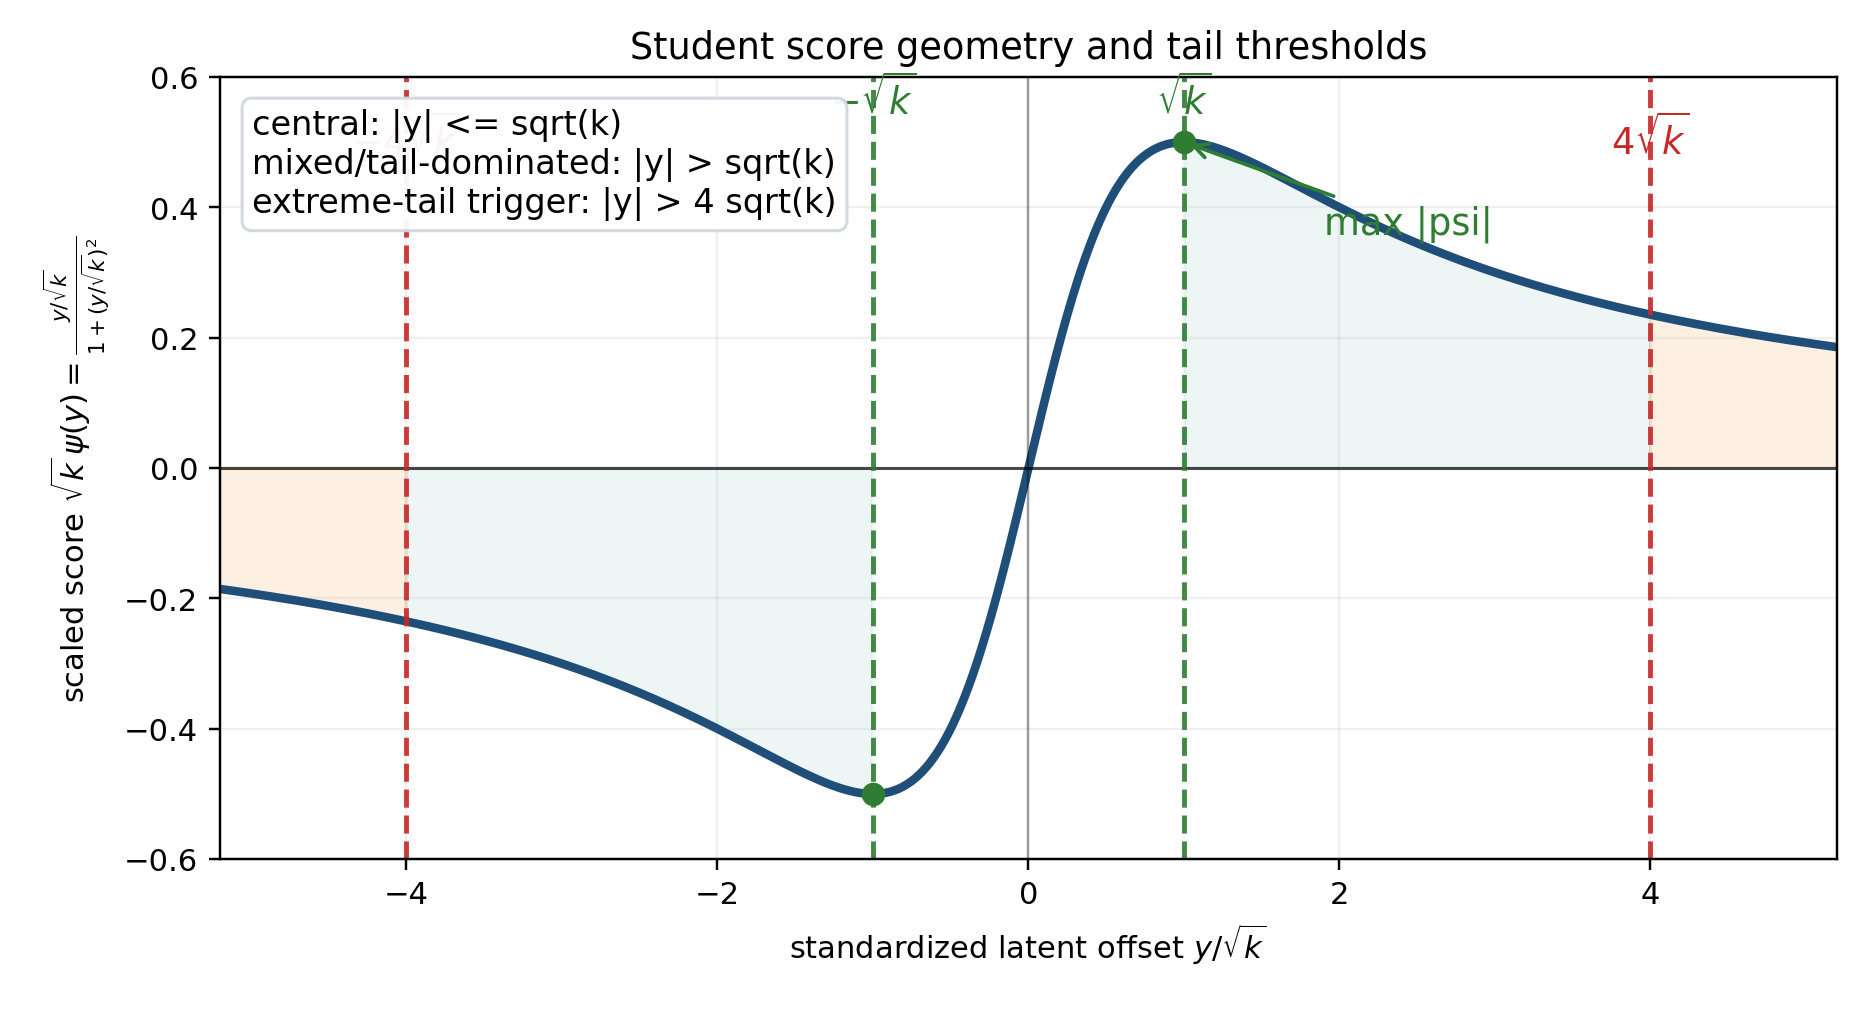
\includegraphics[width=0.72\textwidth]{student_tail_class_definition.png}
  \caption{The two-branch Student score geometry.  The threshold
  $|y|=\sqrt{k}$ is a geometric turning point of $\psi$, not a universal
  outlier threshold.}
  \label{fig:student_score_geometry}
\end{figure}

\subsection{What the current algorithm targets}

Equations~\eqref{eq:pushforward_q}--\eqref{eq:branch_weight} describe the
implemented Student latent update.  Together with the parameter block, they
leave invariant the score-conditioned augmentation
\begin{equation}
 \Pi_{\mathrm{score}}(d\mu,dx)
 \propto \pi_0(\mu)f_\mu(x)
 \frac{1}{\|\nabla_x C(x;\mu^\star)\|}
 \mathbf 1\{C(x;\mu^\star)=0\}
 \,d\mu\,d\Haus^{n-1}(x).
 \label{eq:score_target}
\end{equation}
For exact conditioning on the selected MLE, the Student latent block must also
account for the scalar version of
equation~\eqref{eq:estimating_equation_correction},
\begin{equation}
 R_{\mathrm{MLE}}(x)=
 \left|\sum_{i=1}^n\psi'(x_i-\mu^\star)\right|
 \mathbf 1\{\mu^\star\text{ is the selected MLE for }x\}.
 \label{eq:student_mle_factor}
\end{equation}
This factor couples the branch choices and can be included in a joint pairwise
Metropolis ratio or another exact correction step.

\draftnote{Do not describe the current chain as an exact MLE-conditional chain
until equation~\eqref{eq:student_mle_factor} has been incorporated or proved
irrelevant under stated assumptions.  Re-run the posterior-reference and
privacy experiments after this target is frozen.}

\subsection{Other location models}

For the logistic model, $\psi(y)=\tanh(y/2)$ is monotone and has a single
inverse branch; the same pairwise score-preserving idea is therefore simpler.
For the Laplace model, the MLE is the sample median and the constraint is
order-based rather than a smooth level set.  With odd $n$, the Gibbs update
pins one order statistic at $\mu^\star$ and samples the remaining observations
on the appropriate truncated sides.  This provides a useful example where a
model-specific Gibbs update remains available but smooth-manifold RATTLE is
not directly applicable.

\todo{Write the logistic and odd-$n$ Laplace conditional kernels in full after
the exact estimator-versus-score target audit.  Keep the even-$n$ median
interval convention separate from the unique-median results.}

\section{Invariance, convergence, and a fixed time budget}
\label{sec:convergence}

\subsection{What can be established directly}

For the score-conditioned Student target, the pairwise Metropolis step is
reversible in $z$ space with respect to
equation~\eqref{eq:pair_z_target}; the branch draw is the corresponding exact
conditional draw under the change of variables; and random pairing composes
conditional kernels that share the same invariant target.  The parameter
Metropolis block is invariant for $\pi(\mu\mid x)$.  These observations give a
straightforward invariance argument for equation~\eqref{eq:score_target}.

Invariance is not a convergence theorem.  Harris irreducibility and
aperiodicity require that the combination of random pairings, score proposals,
and branch changes can reach all relevant parts of the target support.  The
Student manifold contains turning points where $\psi'(y)=0$, and the selected
MLE restriction may remove or separate regions.  A complete proof must
characterize these components and show that the pair kernel communicates
between them with positive probability.

\draftnote{Theory options, in increasing strength: (i) prove invariance only;
(ii) prove irreducibility on a regular connected component; (iii) prove
geometric or subgeometric ergodicity under a compact/truncated regime; (iv)
give a regeneration or minorization argument for the one-dimensional
transformed pair kernel.  Do not promise geometric ergodicity in Cauchy-like
tails without a dedicated drift analysis.}

\subsection{Practical monitoring}

Every reported run should monitor quantities tied to the actual transition,
not only generic trace summaries:
\begin{enumerate}
  \item the global constraint residual after each retained sweep;
  \item the before/after pair identity
  $\psi(y_i)+\psi(y_j)=\psi(y_i')+\psi(y_j')$;
  \item transformed-coordinate acceptance, parameter acceptance, inverse-branch
  occupancy and switching, and extreme-residual summaries;
  \item rank-normalized split $\widehat R$, bulk and tail effective sample size,
  Monte Carlo standard errors, and multiseed agreement
  \citep{vehtari2021}; and
  \item sensitivity to central, tail-heavy, and random valid initializations.
\end{enumerate}
For a generic manifold sampler we additionally monitor projection failures,
constraint and tangency residuals, reverse-projection failures, and Hamiltonian
error.  Posterior agreement with an independent reference is necessary but
does not replace these kernel-specific checks.

\subsection{Computation as part of the estimand}

Comparisons will use a pre-specified wall-clock budget $B$ after compilation
and warm-up.  We report seconds per iteration, effective samples per second,
and Monte Carlo error for both parameter and tail-sensitive latent
functionals.  Compilation time, tuning time, and failed projections are
reported separately rather than silently discarded.  The same number of
iterations is not an equal-cost comparison, while ESS per second from a very
short chain is not evidence of convergence.  The final design therefore uses
a short tuning stage followed by multiple fixed-budget production chains.

\todo{Choose $B$, number of seeds, warm-up fraction, thinning policy for latent
storage, and stopping rules before the final rerun.  The parameter chain should
not be declared converged when latent tail indicators remain sticky.}

\section{Why ordinary algorithms struggle with an exact constraint}
\label{sec:comparators}

An unconstrained random-walk or Hamiltonian proposal lands on
$\mathcal M_{t^\star}$ with probability zero.  Three common workarounds change
the problem or require additional correction:
\begin{enumerate}
  \item a tolerance $\|T(x)-t^\star\|\leq\epsilon$ produces an ABC-type
  approximation whose answer depends on $\epsilon$;
  \item a penalty concentrates mass near the manifold but is stiff for small
  tolerances and does not target exact conditioning at a fixed penalty; and
  \item projection back to the manifold changes proposal volumes and can be
  non-unique, so reversibility and Jacobian terms must be handled explicitly.
\end{enumerate}

RATTLE and related constrained-Hamiltonian schemes are principled comparators
for smooth constraints.  Correct implementations use the appropriate surface
target, project momentum to the tangent space, reject failed projections, and
perform a reverse-projection check when required \citep{lelievre2019}.  They
can make global moves unavailable to local Gibbs updates, but their cost and
stability depend on curvature, step size, and the conditioning of the
constraint Jacobian.  They are not directly applicable to the non-smooth
Laplace median constraint.  These facts motivate a comparison rather than a
presumption that either generic geometry or model-specific algebra must win.

\section{Simulation study}
\label{sec:simulation}

\subsection{Questions and design}

The simulation study is organized around four questions:
\begin{enumerate}
  \item \emph{Target correctness:} does each sampler reproduce an independent
  reference for the same conditioning event?
  \item \emph{Weak sufficiency:} how close are
  $\pi(\mu\mid X)$ and $\pi(\mu\mid T(X))$ over repeated datasets?
  \item \emph{Disclosure:} how does releasing $T(X)$ change posterior beliefs
  about latent extremes?
  \item \emph{Computation:} under an equal warmed time budget, which sampler
  produces reliable information fastest?
\end{enumerate}

The normal known-variance model supplies an exact sufficient-statistic
baseline.  Logistic location supplies a smooth monotone score, Student
location with $k\in\{1,2,3\}$ varies tail and branch geometry, and odd-sample
Laplace location supplies a non-smooth median constraint.  The planned sample
sizes are $n\in\{10,20,50\}$ where the estimator convention permits them, with
odd $n\in\{11,21,51\}$ for Laplace.  The Cauchy case $k=1,n=10$ is a diagnostic
stress test until target selection and convergence are resolved.

For location families, equivariance permits an independent likelihood
reference: simulate many centered datasets, compute their selected MLEs, and
use the resulting error distribution to evaluate
$p_T(t^\star\mid\mu)$.  Posterior summaries are computed from raw weighted
Monte Carlo particles.  Kernel density estimation is used only to draw density
overlays.  Bandwidth and kernel choices can strongly affect apparent tail
behavior, so no numerical posterior conclusion is based only on a smoothed
curve.

\subsection{Metrics}

For posterior accuracy we report mean and standard deviation, central and tail
quantiles, interval widths, Wasserstein distance, and Kolmogorov--Smirnov
distance relative to the raw weighted reference.  For weak sufficiency these
are paired full-data versus MLE-only comparisons over simulated datasets, not
a comparison at a single convenient release value.  For disclosure we report
equation~\eqref{eq:privacy_shift} across several prior-predictive percentile
thresholds and include posterior summaries of $\max_i|X_i-t^\star|$.

\subsection{Preliminary evidence and claims not yet frozen}

The existing 100-dataset-per-regime audit recovers the exact normal baseline:
the full-data and MLE-only posteriors agree to numerical precision.  In the
current logistic and Student $k=2,3$ experiments, typical differences are
small and generally decrease with sample size, while small-sample and heavier
tail regimes show larger dispersion and tail differences.  These findings
support studying weak sufficiency as a regime-dependent question rather than a
binary label.

The latent chains also show that conditioning on a central Student MLE does not
force all compatible datasets to be central.  In Cauchy experiments, very
large residuals coexist with bounded score coordinates.  This is the most
direct mechanism through which the released robust estimate can be
insensitive to an observation while the conditional latent-data distribution
still assigns appreciable mass to extreme samples.

\begin{figure}[t]
  \centering
  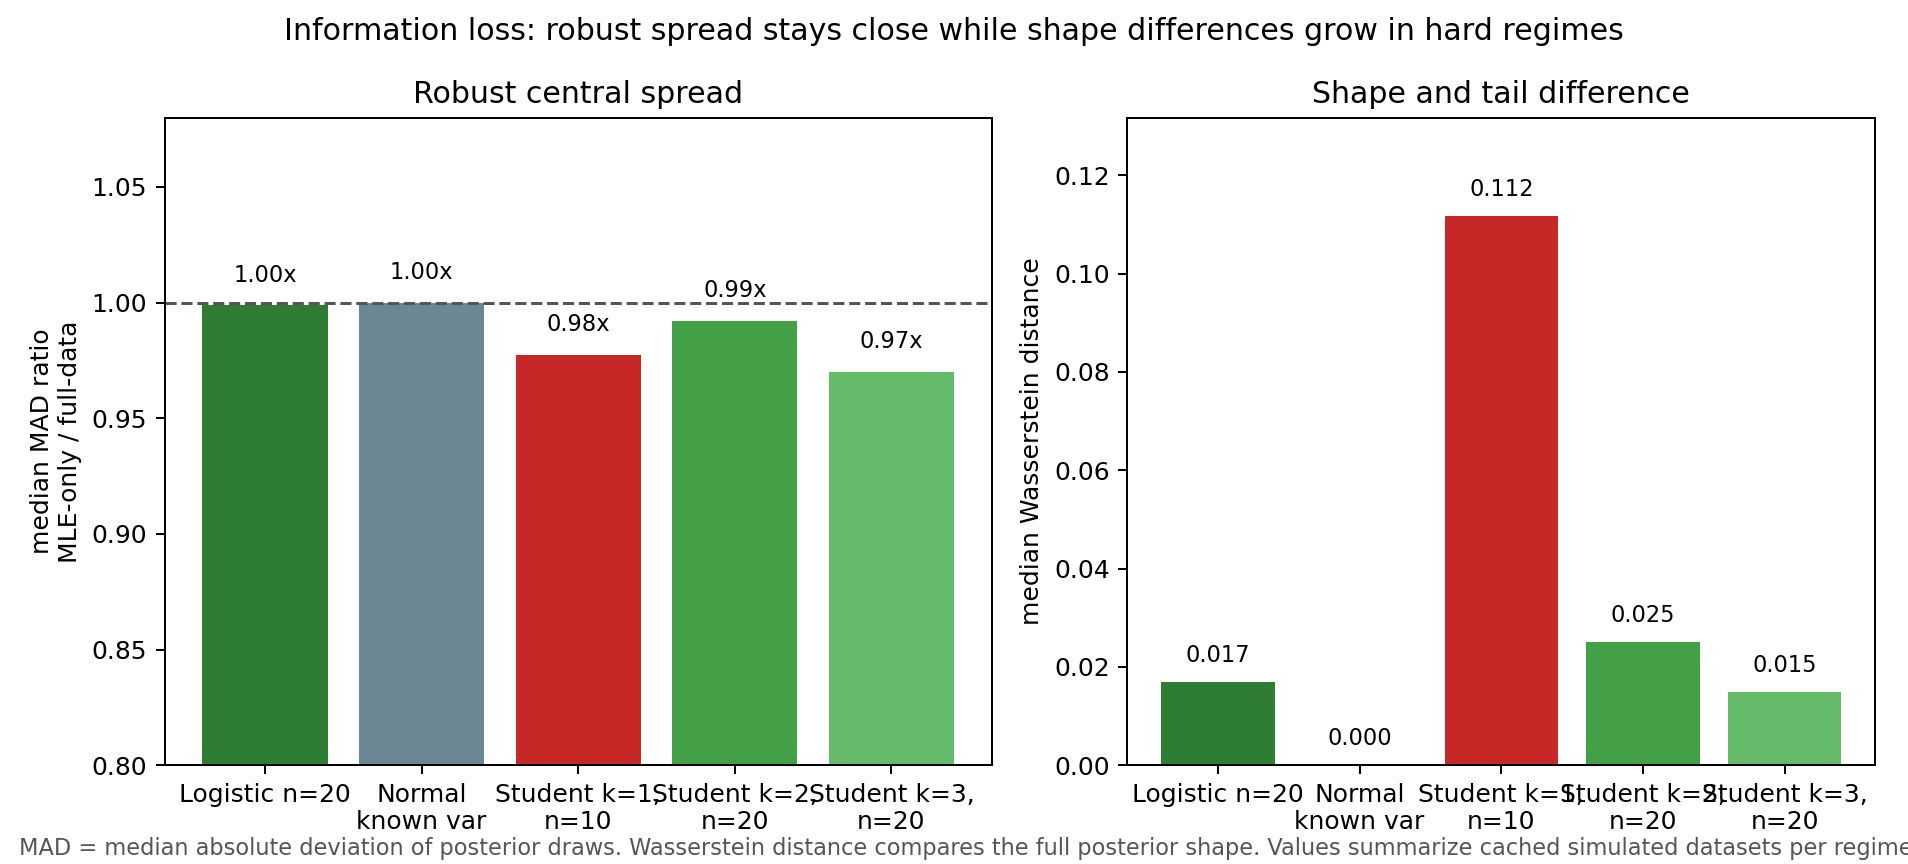
\includegraphics[width=0.78\textwidth]{information_loss_selected_bars.png}
  \caption{Preliminary paired comparison of full-data and MLE-only posterior
  summaries in selected regimes.  Regenerate after freezing the exact-MLE
  target and label the number of datasets and uncertainty across datasets.}
  \label{fig:preliminary_information_loss}
\end{figure}

\begin{figure}[t]
  \centering
  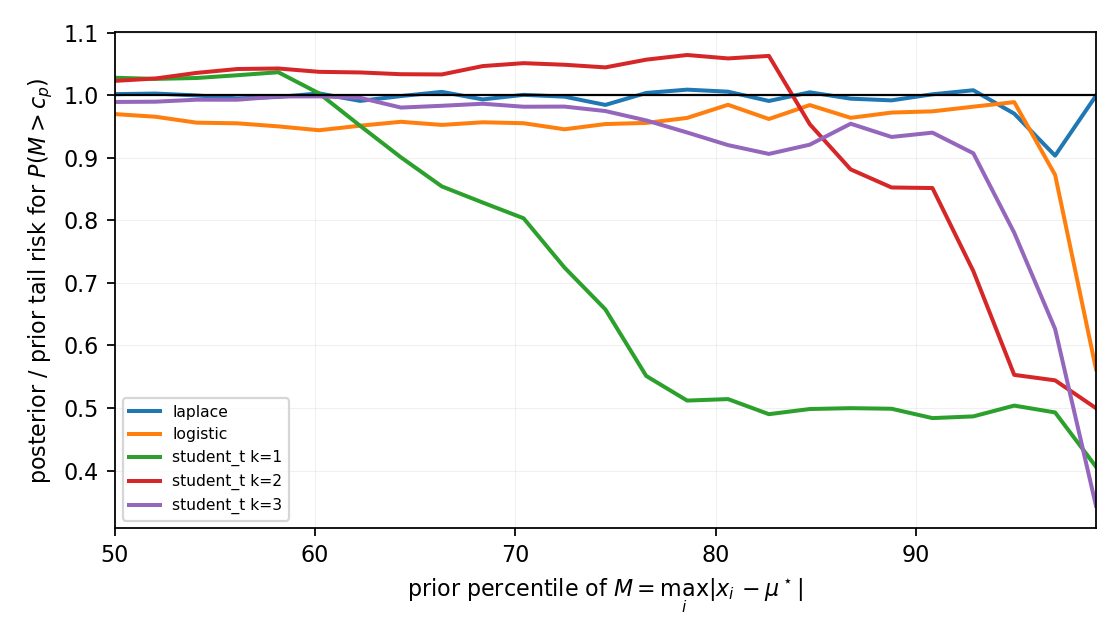
\includegraphics[width=0.78\textwidth]{privacy_leakage_probability_shift.png}
  \caption{Preliminary prior-to-posterior shifts for latent extreme-data
  events.  These are inferential-disclosure summaries, not differential
  privacy guarantees or re-identification probabilities.}
  \label{fig:preliminary_privacy}
\end{figure}

\draftnote{All preliminary sampler-based claims must be regenerated after the
exact selected-MLE target audit.  Existing long-chain evidence can guide the
design, but the older meeting deck's efficiency ranking should not be copied:
the Gibbs implementation has since been replaced by a much faster compiled
kernel.  Use long-chain correctness and warmed timing from the same code
version.}

\section{Discussion}
\label{sec:discussion}

An MLE release sits between two familiar extremes.  A sufficient statistic can
retain all model-based information about the parameter, while a formally
private randomized mechanism controls worst-case changes under neighboring
datasets.  A generic MLE has neither property.  Its practical value and its
disclosure risk depend on the model, estimator geometry, sample size, prior,
and the downstream functional.

Robust scores sharpen this tension.  Bounded or redescending influence is
desirable when the inferential target is a stable location estimate.  The same
compression can erase which observations were extreme, creating many latent
datasets compatible with the release.  That is information loss from the
perspective of full-data Bayes.  At the same time, the release can shift the
probability assigned to particular latent tail events, which is inferential
disclosure.  Neither phenomenon is summarized adequately by the dimension of
the released statistic.

The geometric formulation provides both an algorithm and a warning.  Exact
conditioning on a continuous statistic requires the induced surface measure,
not merely membership in a constraint set.  When an MLE is represented by its
first-order condition, the observed-Hessian and root-selection terms determine
whether the target is truly MLE conditional.  This distinction is mild for
some monotone scores and consequential for redescending scores with multiple
stationary points.

\section{Immediate research roadmap}
\label{sec:roadmap}

\subsection*{Priority 0: freeze the statistical target}
\begin{enumerate}
  \item Prove the coarea expression for the selected MLE under the exact
  conventions used by each model.
  \item For Student location, implement or otherwise account for
  $R_{\mathrm{MLE}}(x)$ in equation~\eqref{eq:student_mle_factor}.
  \item Test score-root, local-maximum, and selected-global-MLE events on every
  retained latent draw; compare the corrected posterior with direct simulated
  MLE references.
\end{enumerate}

\subsection*{Priority 1: establish transition-level correctness}
\begin{enumerate}
  \item Cache the actual before/after pair-$\delta$ error rather than comparing
  thinned snapshots.
  \item Unit-test the truncated-normal Hastings correction and inverse-branch
  probabilities against independent numerical integration.
  \item State and prove the strongest defensible invariance and irreducibility
  result, with singular points and disconnected components explicit.
\end{enumerate}

\subsection*{Priority 2: rerun the evidence hierarchy}
\begin{enumerate}
  \item Posterior correctness against raw weighted-MLE Monte Carlo.
  \item Multiseed and multi-initialization convergence under a fixed time
  budget, including latent tail ESS and Monte Carlo error.
  \item Full-data versus MLE-only paired simulations for weak sufficiency.
  \item Prior-to-posterior latent-event shifts for disclosure, with uncertainty
  across thresholds and datasets.
  \item Gibbs versus RATTLE using the current compiled implementations; keep
  Laplace Gibbs-only unless a valid non-smooth comparator is developed.
\end{enumerate}

\subsection*{Priority 3: final exposition}
Replace draft notes with formal propositions, freeze a small set of main
figures, move tuning and extended diagnostics to the supplement, and shorten
the introduction once the main theorem and empirical message are known.

\begin{thebibliography}{99}

\bibitem[Blackwell(1953)]{blackwell1953}
Blackwell, D. (1953).
Equivalent comparisons of experiments.
\emph{The Annals of Mathematical Statistics}, \textbf{24}, 265--272.

\bibitem[Brubaker et al.(2012)]{brubaker2012}
Brubaker, M., Salzmann, M. and Urtasun, R. (2012).
A family of MCMC methods on implicitly defined manifolds.
\emph{Proceedings of AISTATS}, \textbf{22}, 161--172.

\bibitem[Dwork et al.(2006)]{dwork2006}
Dwork, C., McSherry, F., Nissim, K. and Smith, A. (2006).
Calibrating noise to sensitivity in private data analysis.
\emph{Theory of Cryptography Conference}, 265--284.

\bibitem[Graham and Storkey(2017)]{graham2017}
Graham, M. M. and Storkey, A. J. (2017).
Asymptotically exact inference in differentiable generative models.
\emph{Proceedings of AISTATS}, \textbf{54}, 499--508.

\bibitem[Huber(1964)]{huber1964}
Huber, P. J. (1964).
Robust estimation of a location parameter.
\emph{The Annals of Mathematical Statistics}, \textbf{35}, 73--101.

\bibitem[Leli\`evre et al.(2019)]{lelievre2019}
Leli\`evre, T., Rousset, M. and Stoltz, G. (2019).
Hybrid Monte Carlo methods for sampling probability measures on submanifolds.
\emph{Numerische Mathematik}, \textbf{143}, 379--421.

\bibitem[Marin et al.(2012)]{marin2012}
Marin, J.-M., Pudlo, P., Robert, C. P. and Ryder, R. J. (2012).
Approximate Bayesian computational methods.
\emph{Statistics and Computing}, \textbf{22}, 1167--1180.

\bibitem[Tanner and Wong(1987)]{tanner1987}
Tanner, M. A. and Wong, W. H. (1987).
The calculation of posterior distributions by data augmentation.
\emph{Journal of the American Statistical Association}, \textbf{82}, 528--540.

\bibitem[Vehtari et al.(2021)]{vehtari2021}
Vehtari, A., Gelman, A., Simpson, D., Carpenter, B. and B\"urkner, P.-C. (2021).
Rank-normalization, folding, and localization: An improved $\widehat R$ for
assessing convergence of MCMC.
\emph{Bayesian Analysis}, \textbf{16}, 667--718.

\bibitem[Zappa et al.(2018)]{zappa2018}
Zappa, E., Holmes-Cerfon, M. and Goodman, J. (2018).
Monte Carlo on manifolds: Sampling densities and integrating functions.
\emph{Communications on Pure and Applied Mathematics}, \textbf{71}, 2609--2647.

\end{thebibliography}


\end{document}
